\documentclass{article}

\usepackage{color}
\usepackage{url}
\usepackage[OT2,OT1]{fontenc}
\usepackage[utf8]{inputenc}
\usepackage{graphicx}

\usepackage[english,serbianc]{babel}
\renewcommand{\rmdefault}{wncyr}
\newcommand{\lat}{\fontencoding{OT1}\fontfamily{cmr}\selectfont}

\usepackage[unicode]{hyperref}
\hypersetup{colorlinks}

\usepackage{amsmath}
\usepackage{amssymb}
\usepackage{amsthm}

\newtheorem{teorema}{Teorema}[section]
\newtheorem{lema}{Lema}[section]
\newtheorem{napomena}{Napomena}[section]
\theoremstyle{definition}
\newtheorem{definicija}{Definicija}[section]
\newtheorem{primer}{Primer}[section]

\title{Rekurentne relacije i algoritamska paradigma \emph{podeli pa vladaj}}
\author{Konstantin Ranisavljevic1 \\ Broj indeksa: 186/2025 \\ Matematichki fakultet \\ Univerzitet u Beogradu}
\date{\today}

\begin{document}
\maketitle
\tableofcontents

\section*{Uvod}
Mnoge aktivnosti bez kojih danashnju svakodnevicu ne bismo mogli ni zamisliti izvrshavamo brzhe nego ikada pre. To nam danas o\-mo\-gu\-c1a\-va\-ju rachunari i njima prilagodjeni algoritmi koji su nekada predstavljali dosta sporije procedure. Ipak, primec1ujemo da, kako slozhenost ovih algoritama i kolichina podataka koji u njima uchestvuju rastu, raste i kolichina vremena potrebna da se pomenuti algoritmi izvrshe. Zato, na primer, svi sistemi velikih kompanija zavise od algoritama koji su optimizovani da nam rezultate daju velikom br\-zi\-nom.


Bez odgovarajuc1e analize algoritama, ovi sistemi bili bi pre\-spo\-ri, a osim toga i energet{}ski vrlo neefikasni, te preskupi. Ovaj problem chesto reshava posebna vrsta algoritama koji se zasnivaju na algoritamskoj paradigmi \emph{podeli pa vladaj}, a matematichki model koji ih precizno objashnjava jesu rekurentne relacije.

\section{Rekurentne relacije}
Rekurentne relacije definishu niz u zavisnosti od njegovih pret\-hod\-nih chlanova.

\begin{definicija}
Neka je $\{a_n\}_{n\in\mathbb{N}}$ niz realnih brojeva. Rekurentna relacija reda $k\in\mathbb{N}$ je jednachina oblika $$a_n = f(n, a_{n-1}, a_{n-2}, \ldots, a_{n-k})\quad \text{za}\quad n\geqslant k,$$ pri chemu je $f:\mathbb{N}\times X^k \to X$ funkcija koja ukljuchuje $k$ uzastopnih chlanova niza, a $X$ skup kome pripadaju svi chlanovi niza.
\end{definicija}

\begin{napomena}
Rekurentna relacija je jednoznachno odredjena ako je zadato $k$ inicijalnih vrednosti $a_0,a_1,\ldots,a_{k-1}$. Bez zadatih inicijalnih vred\-no\-sti, relacija opisuje beskonachnu familiju nizova.
\end{napomena}

\begin{primer}
Faktorijel je definisan rekurentnom relacijom $$n! = n\cdot(n-1)!\quad\text{za}\quad n>0$$ i inicijalnom vrednosh{}c1u $0! = 1$.
\end{primer}

\begin{primer}
Fibonachijevi brojevi pripadaju nizu chiji je svaki chlan zbir prethodna dva chlana. Fibonachijev niz je definisan rekurentnom relacijom $$F_n = F_{n-1} + F_{n-2}$$ i inicijalnim vrednostima $F_0 = 0$ i $F_1 = 1$. Prvih nekoliko chlanova Fibonachijevog niza jesu: $0,1,1,2,3,5,8,13,21,34,55,89,\ldots$
\end{primer}

\begin{definicija}
Rekurentna relacija je \emph{linearna} ako je $$a_n = \sum_{i=1}^{k} c_i a_{n-i} + g(n),$$ pri chemu su $c_i$ konstante ili funkcije od $n$, a $g(n)$ slobodan chlan.
\end{definicija}

\begin{definicija}
Linearna rekurentna relacija je \emph{homogena} ako je $g(n) = 0$, a inache je \emph{nehomogena}.
\end{definicija}

\begin{lema}[Linearnost]
Neka su $\{a_n\}$ i $\{b_n\}$ reshenja homogene linearne rekurentne relacije $x_n = \sum_{i=1}^{k} c_i x_{n-i}$. Tada je za sve konstante $\alpha,\beta\in\mathbb{R}$ niz $$u_n = \alpha a_n + \beta b_n$$ takodje reshenje iste rekurentne relacije.
\end{lema}

\begin{proof}
Pretpostavimo da su $\{a_n\}$ i $\{b_n\}$ reshenja relacije $\{x_n\}$. To znachi da se mogu zapisati kao $a_n = \sum_{i=1}^{k} c_i a_{n-i}$ i $b_n = \sum_{i=1}^{k} c_i b_{n-i}$.
Za $n\geqslant k$ i $\alpha,\beta\in\mathbb{R}$ definishimo novi niz
\begin{eqnarray*}
u_n = \alpha a_n + \beta b_n & = & \alpha(c_1 a_{n-1} +\cdots + c_k a_{n-k})+\beta(c_1 b_{n-1} +\cdots + c_k b_{n-k}\\
& = & c_1(\alpha a_{n-1}+\beta b_{n-1}) + \cdots + c_k(\alpha a_{n-k} + \beta b_{n-k})\\
& = & c_1 u_{n-1} + c_2 u_{n-2} + \cdots + c_k u_{n-k}.
\end{eqnarray*}
Niz $\{u_n\}$ zadovoljava istu rekurentnu relaciju, te je i on njeno reshenje.
\end{proof}

\emph{Reshiti rekurentnu relaciju} znachi nac1i eksplicitnu formulu za opshti chlan niza. Neki od nachina reshavanja su:
\begin{itemize}
\item iterativna metoda (npr. $a_{n-1}$ se izrazi preko $a_{n-2}$);
\item metoda karakteristichne jednachine (uz pretpostavku $a_n = r^n$);
\item pomoc1u master teoreme (teorema \ref{thm:master}) i
\item pomoc1u rekurzivnog stabla (slika \ref{fig:rekurzivno_stablo}).
\end{itemize}

\begin{figure}[h]
\centering
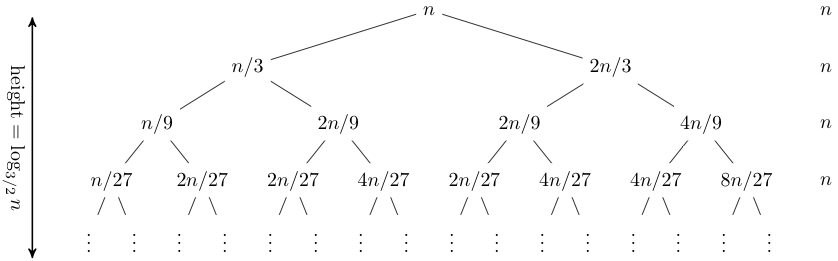
\includegraphics[scale=0.8]{recursiontree.png}
\caption{Rekurzivno stablo}
\label{fig:rekurzivno_stablo}
\end{figure}

\section{Algoritamska paradigma {\lat\quotedblbase}podeli pa vladaj”}
\subsection{Algoritmika}
\emph{Algoritmika} je oblast informatike koja se bavi analizom vre\-men\-ske i prostorne slozhenosti programa, kao i dizajnom shto efikasnijih algoritama koji reshavaju neki problem. \emph{Algoritamska slozhenost} je funkcija koja opisuje kako resursi koje algoritam troshi zavise od velichine ulaza. Resursi su uglavnom vreme izvrshavanja, memorija i energija. \emph{Velichina ulaza} $n$ je mera kolichine informacija koje al\-go\-ri\-tam prima i najchesh{}c1e predstavlja broj bitova u broju, broj elemenata u nizu, broj chvorova u grafu ili duzhinu niske. \emph{Asimptot{}ska notacija} opisuje ponashanje funkcije kada $n\to\infty$, zanemarujuc1i konstante i nizhe redove.

\begin{definicija}
Neka su $f$ i $g$ dve pozitivne funkcije od $n\in\mathbb{N}$. Za funkciju $g(n)$ kazhe se da je \emph{asimptot{}ska gornja granica} funkcije $f(n)$ i pishe se $f(n) = \mathcal{O}\big(g(n)\big)$ ako postoje pozitivne konstante $c$ i $n_0$ takve da za svako $n>n_0$ vazhi $f(n) \leqslant cg(n)$.
\end{definicija}

\begin{definicija}
Za funkciju $g(n)$ kazhe se da je \emph{asimptot{}ska donja granica} funkcije $f(n)$ i pishe se $f(n) = \Omega\big(g(n)\big)$ ako postoje pozitivne konstante $c$ i $n_0$ takve da za svako $n>n_0$ vazhi $f(n) > cg(n)$.
\end{definicija}

\begin{definicija}
Ako za dve funkcije $f$ i $g$ vazhi $f(n) = \mathcal{O}\big(g(n)\big)$ i $f(n) = \Omega\big(g(n)\big)$, onda za funkciju $g(n)$ kazhemo da je \emph{asimptot{}ska tesna granica} funkcije $f(n)$ i pishemo $f(n) = \Theta\big(g(n)\big)$.
\end{definicija}

\begin{definicija}
Za $k>0,\;0<\varepsilon<1$ i $c>1$ definishe se strogo uredjena hijerarhija rasta funkcija $$1 \ll \log n \ll \log^k n \ll n^\varepsilon \ll n \ll n\log n \ll n^2 \ll n^3 \ll \cdots \ll c^n \ll n! \ll n^n.$$
\end{definicija}

\subsection{O paradigmi}
Algoritmi zasnovani na algoritamskoj paradigmi \emph{podeli pa vladaj} (eng. \emph{\lat divide and conquer}) reshavaju problem tako shto ga podele na manje potprobleme iste vrste, a zatim reshe potprobleme da bi na kraju spojili parcijalna reshenja u reshenje problema.

\begin{definicija}
Ako je velichina problema $n$, a algoritam reshava $a\geqslant 1$ potproblema velichine $\frac{n}{b}$ ($b>1$ je faktor smanjenja velichine problema) uz dodatni rad $f(n)$ na podelu i kombinovanje, rekurentna relacija koja opisuje \emph{podeli pa vladaj} algoritme je $$T(n) = aT\Big(\frac{n}{b}\Big) + f(n).$$ Asimptot{}sko reshenje ove rekurentne relacije daje teorema \ref{thm:master}.
\end{definicija}

\begin{teorema}[Master teorema]
\label{thm:master}
Za rekurentnu relaciju $T(n) = aT(\frac{n}{b}) + f(n)$ i $\lambda = \log_b a$ vazhe sledec1a tri sluchaja:
\begin{enumerate}
\item ako je $f(n) = \mathcal{O}(n^{\lambda - \varepsilon})$, tada je $T(n)=\Theta(n^\lambda)$;
\item ako je $f(n) = \Theta(n^\lambda \log^k n)$, tada je $T(n) = \Theta(n^\lambda \log^{k+1} n)$;
\item ako je $f(n) = \Omega(n^{\lambda + \varepsilon})$ i $af(\frac{n}{b}) \leqslant cf(n)$ za neko $c<1$, tada je $T(n) = \Theta\big(f(n)\big)$.
\end{enumerate}
\end{teorema}

U tabeli \ref{tab:poredjenje} dato je poredjenje nekih relevantnih \emph{podeli pa vladaj} algoritama po vremenskoj i prostornoj slozhenosti.

\begin{table}[h]
\centering
\begin{tabular}{c||c|c|c}
\textbf{Algoritam} & \textbf{Rekurentna relacija} & \textbf{Vreme} & \textbf{Prostor}\\ \hline
{\lat Merge Sort} & $T(n) = 2T(\frac{n}{2})+n$ & $\Theta(n\log n)$ & $\Theta(n)$\\
{\lat Quick Sort} & $T(n) = T(k)+T(n-k)+n$ & $\Theta(n\log n)$ & $\mathcal{O}(\log n)$\\
{\lat Binary Search} & $T(n) = T(\frac{n}{2})+1$ & $\Theta(\log n)$ & $\mathcal{O}(1)$
\end{tabular}
\caption{Poredjenje nekih relevantnih algoritama}
\label{tab:poredjenje}
\end{table}

\section*{Zakljuchak}
Velike zasluge za brzinu kojom danas izvrshavamo svakodnevne ak\-tiv\-no\-sti pripadaju algoritmima zasnovanim na paradigmi \emph{podeli pa vladaj} i matematichkom modelu na kome se temelje --- rekurentnim re\-la\-ci\-ja\-ma. U ovom radu je sistematichno objashnjeno kako teorijska sa\-rad\-nja nizova i algoritmike daju praktichno reshenje za vremenski, energet{}ski i fi\-nan\-sij\-ski efikasnije programe.

\end{document}